\begin{frame}{From physics to the mathematical model}
  \vspace{-0.6cm}
  \begin{overprint}
    \onslide<1>
    \begin{columns}
      \begin{column}{0.45\textwidth}
        \begin{block}{Solid dynamics problems}
          \begin{itemize}
          \item[] \textbf{Impact; Crash-proof design}
          \item[] High-speed forming
          \item[] Earthquake reliability of structures 
          \end{itemize}
        \end{block}
      \end{column}
      
      \begin{column}{0.55\textwidth}
      \end{column}
    \end{columns}
    
    \begin{figure}[ht]
      \centering
      \subcaptionbox{Bird strike on aircrafts}{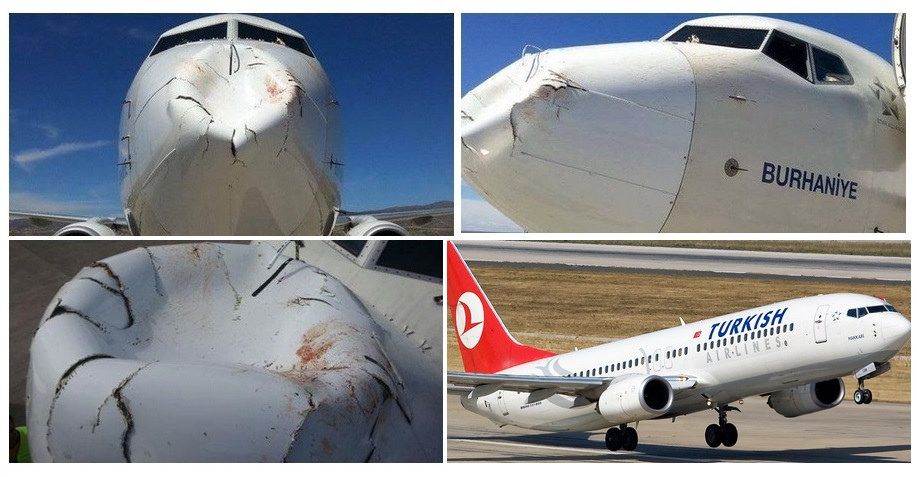
\includegraphics[height=0.3\paperheight]{section1/pictures/birdstrike.jpg}}
      \subcaptionbox{Glasgow Museum of Transport}{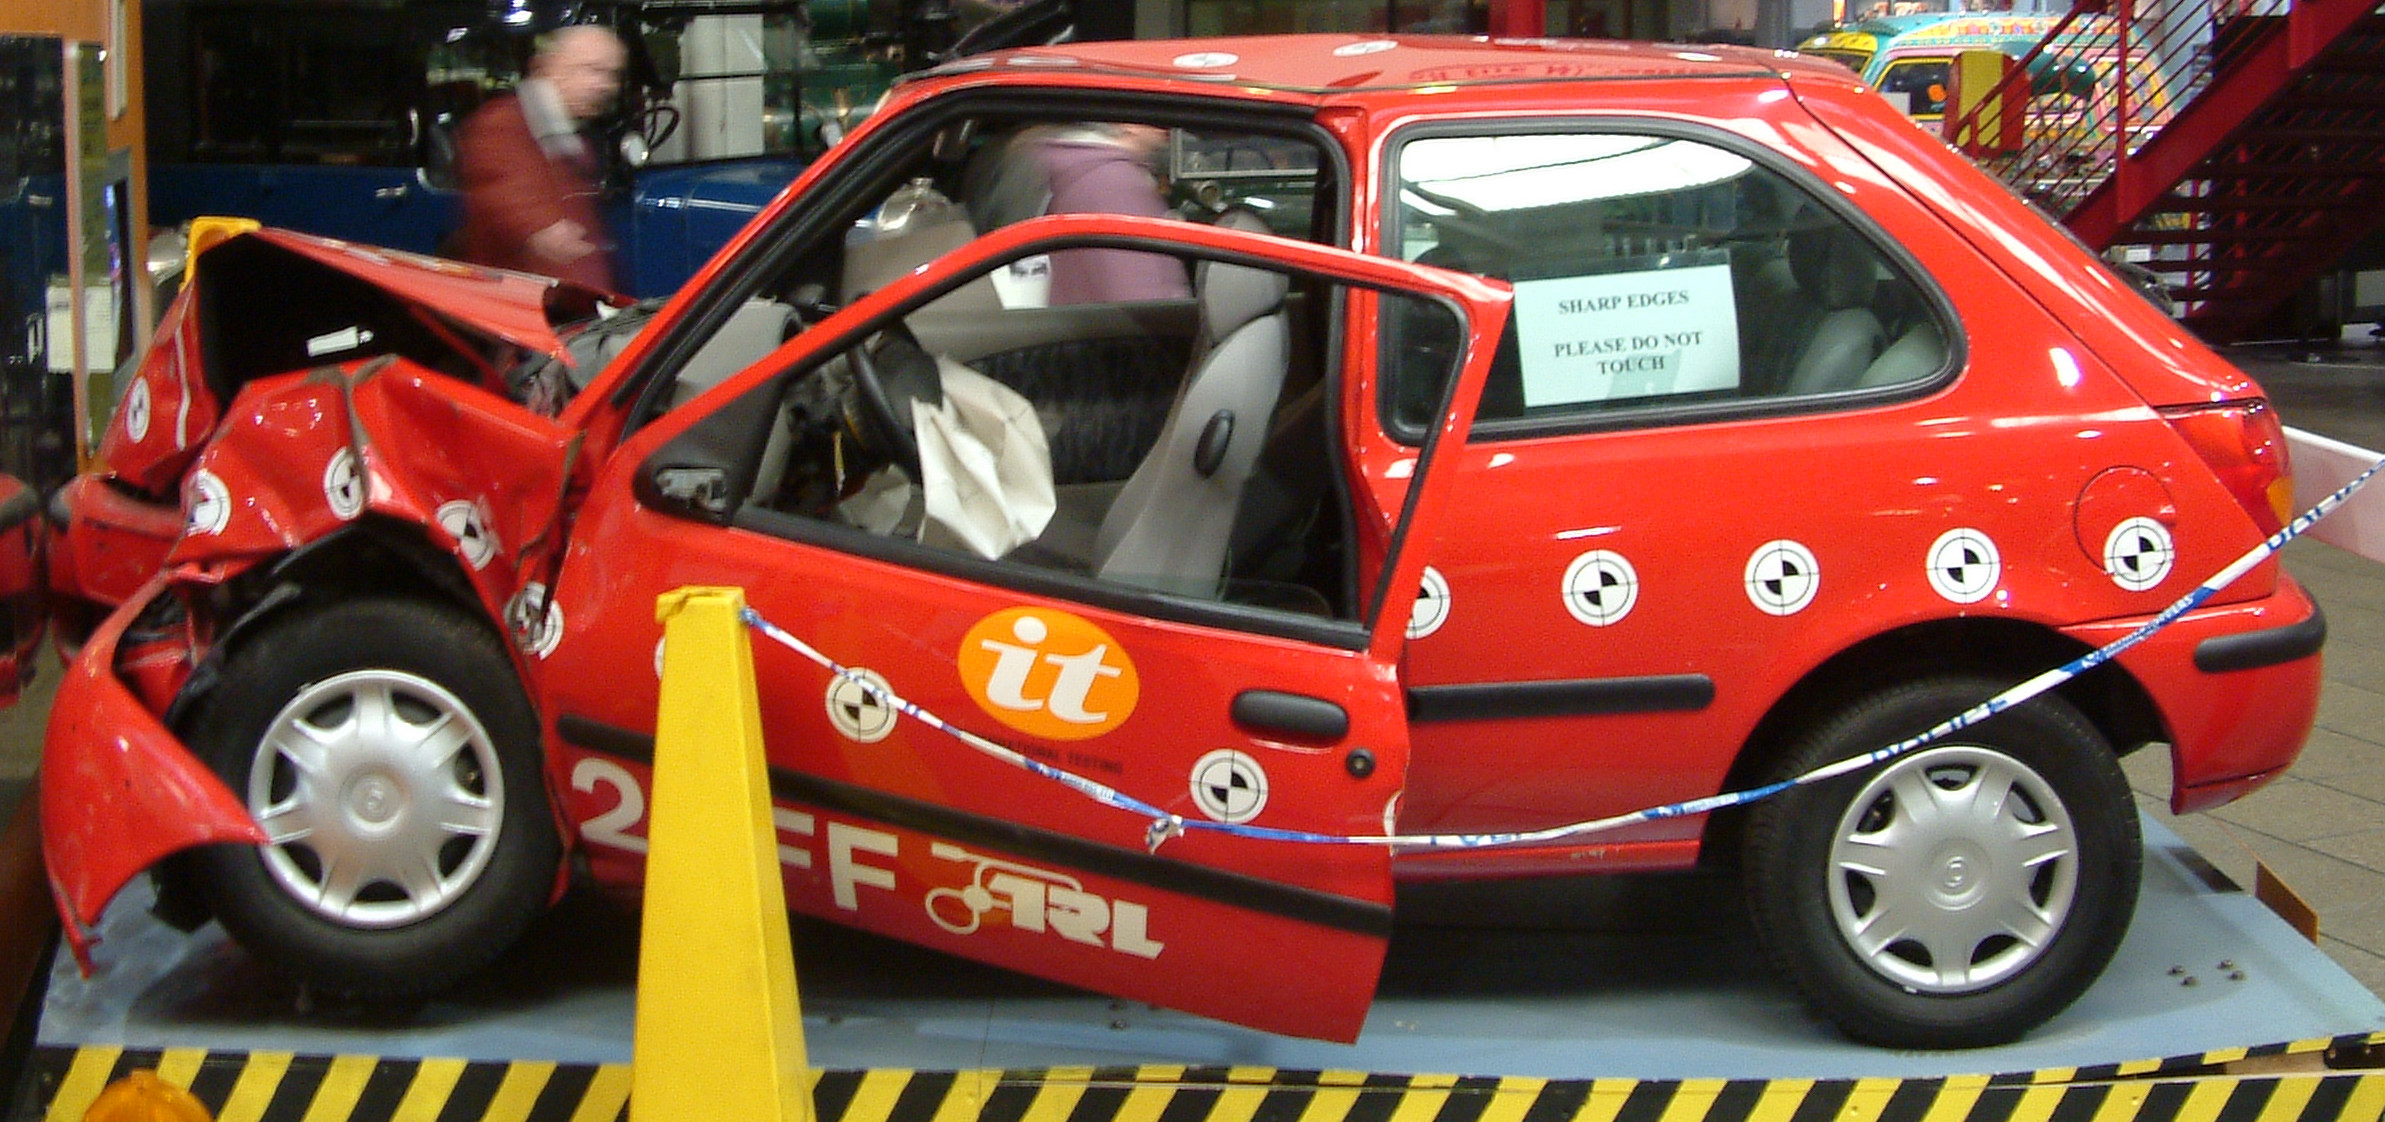
\includegraphics[height=0.3\paperheight]{section1/pictures/crash2.jpg}}
    \end{figure}
    
    \onslide<2>
    \begin{columns}
      \begin{column}{0.45\textwidth}
        \begin{block}{Solid dynamics problems}
          \begin{itemize}
          \item[] Impact; Crash-proof design
          \item[] \textbf{High-speed forming}
          \item[] Earthquake reliability of structures 
          \end{itemize}
        \end{block}
      \end{column}
      
      \begin{column}{0.55\textwidth}
      \end{column}
    \end{columns}

    \centering
    \movie[height = 0.35\paperheight,width=0.25\linewidth,loop,poster,autostart]{}{%
      section1/animation/output3.mp4}\\
    \scriptsize Electromagnetic forming \cite{Formage}
    \vfill
    {\tiny
      \usebibitemtemplate{\color{structure}\insertbiblabel} 
      \usebibliographyblocktemplate{\color{structure}}{\color{black}}{\color{structure!75}}{\color{structure!75}} 
      \begin{thebibliography}{EMF}
        \tiny \bibitem[1]{Formage}
        Bon E.,Priem D.,Sow C., Heuzé T., Racineux G.
        \newblock Electromagnetic bending of an aluminum sheet
        \newblock {\em GeM, Ecole centrale de Nantes, 2015}.
      \end{thebibliography}}  

    \onslide<3>
    \begin{columns}
      \begin{column}{0.45\textwidth}
        \begin{block}{Solid dynamics problems}
          \begin{itemize}
          \item[] Impact; Crash-proof design
          \item[] High-speed forming
          \item[] \textbf{Earthquake reliability of structures}
          \end{itemize}
        \end{block}
      \end{column}
      
      \begin{column}{0.55\textwidth}
      \end{column}
    \end{columns}

    \centering
    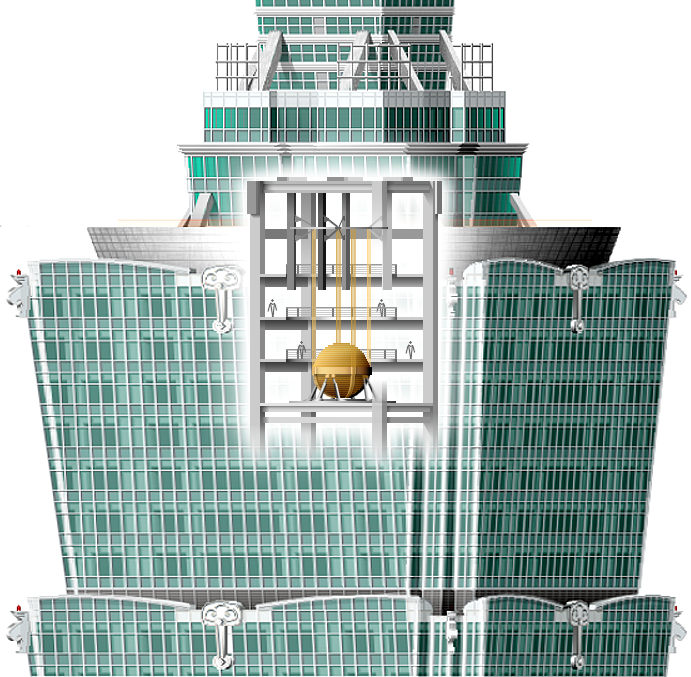
\includegraphics[scale=0.15]{section1/pictures/TaipeiTower.png} \quad
    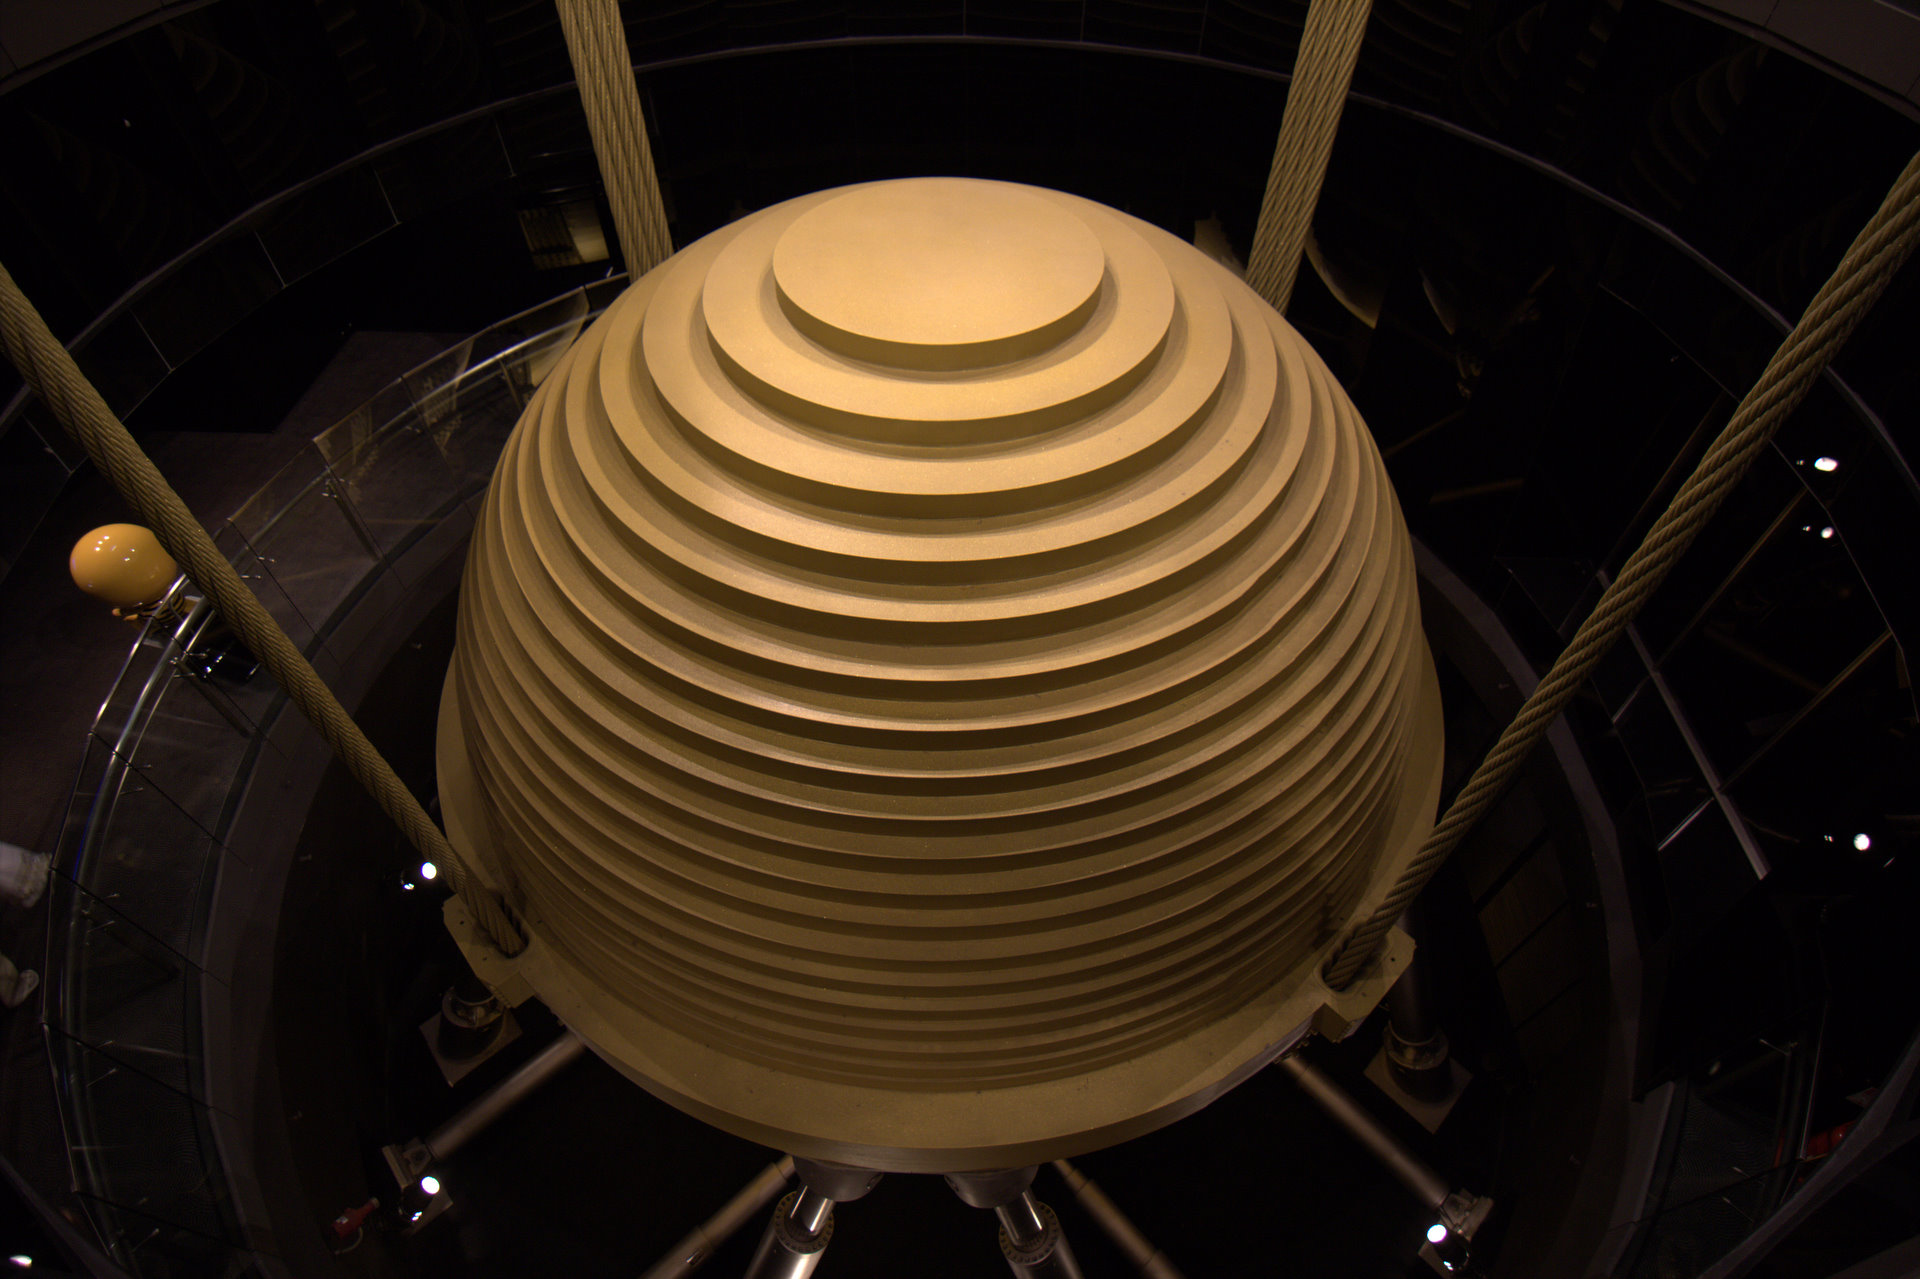
\includegraphics[scale=0.08]{section1/pictures/MassDamper.jpg}\\
    \scriptsize Taipei 101 mass damper

    \onslide<4>
    \begin{columns}
      \begin{column}{0.45\textwidth}
        \begin{block}{Solid dynamics problems}
          \begin{itemize}
          \item[] Impact; Crash-proof design
          \item[] High-speed forming
          \item[] Earthquake reliability of structures 
          \end{itemize}
        \end{block}
      \end{column}
      
      \begin{column}{0.55\textwidth}
        \begin{block}{Partial differential equations}
          \begin{equation*}
            \Rightarrow \left\lvert
              \begin{aligned}
                & \text{Conservation laws} \\
                & \text{Constitutive equations} 
              \end{aligned}
            \right. = \textbf{Hyperbolic system}
            % Préciser les équations dans le dévelopement de la DGMPM
          \end{equation*}
        \end{block}
      \end{column}
    \end{columns}
    
    \begin{block}{Difficulties for the solution of hyperbolic equations:}
      \begin{itemize}
      \item complex geometries
      \item waves propagating/interacting in solids
      \item finite deformations
      \end{itemize}
    \end{block}
    \textbf{$\Rightarrow$ Resort to numerical simulation}
  \end{overprint}
\end{frame}

% Problems considered -- dynamics + applications + solid mechanics (equations)
% Soit (i) on inclue les équations du modèle dans les motivations soit (ii) on parle d'abord des difficultés qu'après on illustre ?

% (i) - Problèmes de dynamique des solides: lois de conservations + lois constitutives => système hyperbolique
% - EDP dont les solutions font intervenir des ondes
% - Equations complexes (non-linéaires + multi-dimensionnelle) + solutions compliquées car ondes qui interagissent
% - Intérêt de la simulation pour calculer des solutions approchées
% - Mais cependant, on a des limitations (grandes defs ; suivi des ondes [oscillations + diffusion] ; difficultées à assurer la convergence vers une solution physique ??? [un truc pour introduire la prise en compte de la structure caractéristique])
% - Exemples de limitations avec les méthodes existantes : FEM -- FV -- Meshfree 

% \begin{frame}{The numerical simulation}
%   \begin{block}{It allows to:}
%     \begin{itemize}
%     \item compute approximate solutions
%     \item highlight phenomena implicitly described by the model
%     \item perform virtual experiments
%     \end{itemize}
%   \end{block}
%   \begin{block}{While struggling with:}
%     \begin{itemize}
%     \item the space discretization (mesh-based or mesh-free techniques)
%     \item the regularity of the problem (discontinuous solutions)
%     \item 
%     \end{itemize}
%   \end{block}
% \end{frame}

\begin{frame}{Suitability of some Lagrangian methods}
  \begin{columns}
    \begin{column}{0.3\textwidth}
      \begin{block}{Finite Element Method}
        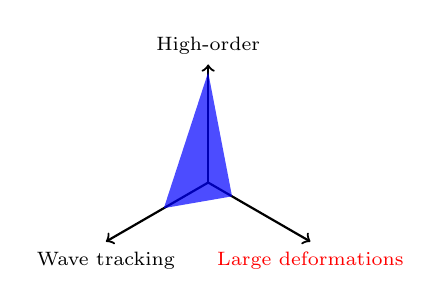
\begin{tikzpicture}
          \draw[->,  thick] (0.,0.) -- (0.,1.5) node[above] {\scriptsize \text{High-order}};
          \draw[->,  thick] (0.,0.) -- (0.8660*1.5,-0.5*1.5) node[below] {\scriptsize \color{Red} \text{Large deformations}};
          \draw[->,  thick] (0.,0.) -- (-0.8660*1.5,-0.5*1.5) node[below] {\scriptsize \text{Wave tracking}};
          \fill[Blue,opacity=0.7] (0,1.40) -- (0.8660*0.35,-0.5*0.35) -- (-0.8660*0.65,-0.5*0.65) -- (0.,1.40);
          % \node at (-1.,1.) {$\text{FEM}$};
        \end{tikzpicture}
      \end{block}
    \end{column}
    \begin{column}{0.3\textwidth}
      \begin{block}{Finite Volume Method}
        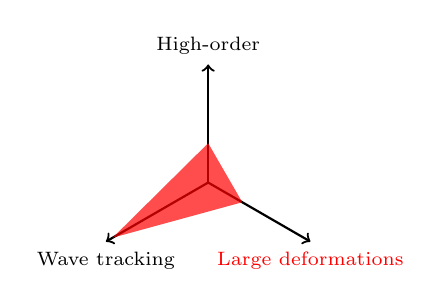
\begin{tikzpicture}
          \draw[->,  thick] (0.,0.) -- (0.,1.5) node[above] {\scriptsize \text{High-order}};
          \draw[->,  thick] (0.,0.) -- (0.8660*1.5,-0.5*1.5) node[below] {\scriptsize \color{Red} \text{Large deformations}};
          \draw[->,  thick] (0.,0.) -- (-0.8660*1.5,-0.5*1.5) node[below] {\scriptsize \text{Wave tracking}};
          \fill[Red,opacity=0.7] (0,.5) -- (0.8660*0.5,-0.5*0.5) -- (-0.8660*1.40,-0.5*1.40) -- (0.,.5);
        \end{tikzpicture}
      \end{block}
    \end{column}
    \begin{column}{0.33\textwidth}
      \begin{block}{Discontinuous Galerkin FEM}
        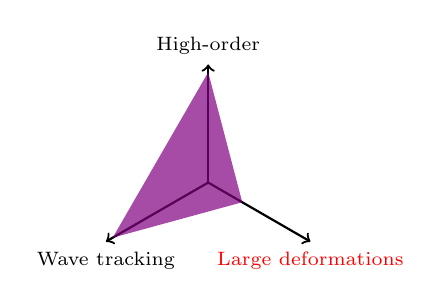
\begin{tikzpicture}
          \draw[->,  thick] (0.,0.) -- (0.,1.5) node[above] {\scriptsize \text{High-order}};
          \draw[->,  thick] (0.,0.) -- (0.8660*1.5,-0.5*1.5) node[below] {\scriptsize \color{Red} \text{Large deformations}};
          \draw[->,  thick] (0.,0.) -- (-0.8660*1.5,-0.5*1.5) node[below] {\scriptsize \text{Wave tracking}};
          \fill[Purple,opacity=0.7] (0,1.40) -- (0.8660*0.5,-0.5*0.5) -- (-0.8660*1.40,-0.5*1.40) -- (0.,1.40);
        \end{tikzpicture}
      \end{block}
    \end{column}
  \end{columns}
\end{frame}

\begin{frame}{Mesh-free Lagrangian approaches: The Material Point Method}
  \begin{columns}
    \begin{column}{0.3\textwidth}
      \begin{block}{Material Point Method}
        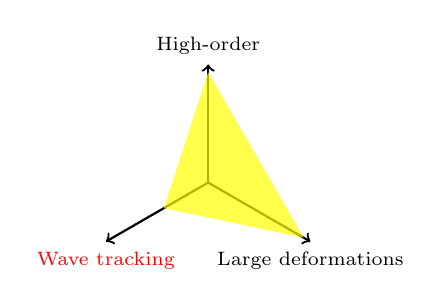
\begin{tikzpicture}
          \draw[->,  thick] (0.,0.) -- (0.,1.5) node[above] {\scriptsize \text{High-order}};
          \draw[->,  thick] (0.,0.) -- (0.8660*1.5,-0.5*1.5) node[below] {\scriptsize \text{Large deformations}};
          \draw[->,  thick] (0.,0.) -- (-0.8660*1.5,-0.5*1.5) node[below] {\scriptsize \color{Red} \text{Wave tracking}};
          \fill[Yellow,opacity=0.7] (0,1.40) -- (0.8660*1.40,-0.5*1.40) -- (-0.8660*.65,-0.5*.65) -- (0.,1.40);
        \end{tikzpicture}
      \end{block}
    \end{column}
    \begin{column}{0.4\textwidth}
      \begin{block}{Discontinuous Galerkin MPM ?}
        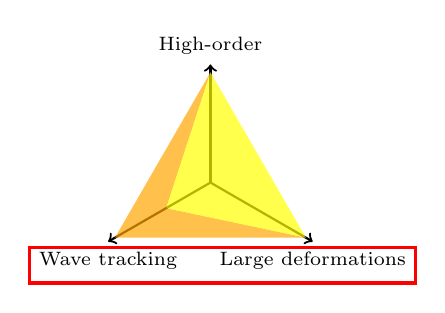
\begin{tikzpicture}
          \draw[->,  thick] (0.,0.) -- (0.,1.5) node[above] {\scriptsize \text{High-order}};
          \draw[->,  thick] (0.,0.) -- (0.8660*1.5,-0.5*1.5) node[below] {\scriptsize \text{Large deformations}};
          \draw[->,  thick] (0.,0.) -- (-0.8660*1.5,-0.5*1.5) node[below] {\scriptsize \text{Wave tracking}};
          \fill[Orange,opacity=0.7] (0,1.40) -- (-0.8660*1.40,-0.5*1.40) -- (0.8660*1.40,-0.5*1.40)--(-0.8660*.65,-0.5*.65) -- (0.,1.40);
          \draw[Red, very thick] (-2.3,-0.85*1.5) rectangle (2.6,-0.55*1.5);
          \fill[Yellow,opacity=0.7] (0,1.40) -- (0.8660*1.40,-0.5*1.40) -- (-0.8660*.65,-0.5*.65) -- (0.,1.40);
        \end{tikzpicture}
        %\animategraphics[autoplay,loop]{1}{section1/animation}{}{}
      \end{block}
    \end{column}
  \end{columns}
  $\newline$
  \metroset{block=fill}
  \begin{block}{Objective 1}
    Merge the advantages of FEM, FVM and MPM by means of the DG approximation
  \end{block}
\end{frame}


% \begin{frame}
%   \metroset{block=fill}
%   \begin{block}{Pros and cons of some mesh-based methods:}
%     \metroset{block=transparent}
%     \begin{footnotesize}
%       \begin{columns}
%         \begin{column}{.45\textwidth}
%           \begin{block}{\footnotesize The Finite Element Method (FEM)}
%             \begin{itemize}
%             \item[$+$] handle nonlinear constitutive models
%             \item[$+$] high-order approximation
%             \item[$-$] oscillations near discontinuities
%             \item[$-$] dealing with large deformations
%             \end{itemize}
%           \end{block}
%         \end{column}
%         \begin{column}{.45\textwidth}
%           \begin{block}{\footnotesize The Finite Volume Method (FVM)}
%             \begin{itemize}
%             \item[$+$] handle nonlinear constitutive models
%             \item[$-$] high-order approximation
%             \item[$+$] removal of oscillations
%             \item[$-$] dealing with large deformations
%             \end{itemize}
%           \end{block}
%         \end{column}
%       \end{columns}
%     \end{footnotesize}
%   \end{block}
% \end{frame}

% \begin{frame}{The numerical simulation}
%   \metroset{block=fill}
%   \begin{normalsize}
%     \begin{block}{The Discontinuous Galerkin approximation: taking advantage of both FEM and FVM}
%       \begin{itemize}
%       \item[$+$] handle nonlinear constitutive models
%       \item[$+$] high-order approximation
%       \item[$+$] removal of oscillations
%         \alert{\item[$-$] \textbf{dealing with large deformations $\rightarrow$ resort to mesh-free methods}}
%       \end{itemize}
%     \end{block}
%     \pause
%     \begin{block}{Particle-in-cell approaches -- the Material Point Method (MPM)}
%       \begin{itemize}
%       \item[$+$] handle nonlinear constitutive models
%       \item[$+$] high-order approximation
%       \item[$-$] numerical oscillations and diffusion
%       \item[$+$] handle large deformation
%       \end{itemize}
%     \end{block}
%   \end{normalsize}
% \end{frame}

\begin{frame}{The simulation is bounded by the model}
  %%
  \begin{block}{Inheritance from fluid dynamics}
    Numerical tools to embed information about the solution in numerical approaches
  \end{block}
  \begin{block}{The point of view adopted here}
    \begin{itemize}
    \item Combine such tools with robust discretization techniques should lead to accurate solutions
    \item Make a numerical approach able to mimic the physical response
    \end{itemize}
  \end{block}
  \begin{block}{Limitations}
    Gaps about some constitutive models (dammage, plasticity, thermo-mechanical coupling etc.)
  \end{block}
  \metroset{block=fill}
  \begin{block}{Objective 2}
    Investigate the response of two-dimensional elastic-plastic solids to dynamic loading
  \end{block}
\end{frame}



%%% Local Variables:
%%% mode: latex
%%% TeX-master: "../aRenaud"
%%% End:
